\section{Experimental Setup and Methodology}
\label{sec:methodology}

\begin{table}[!t]
\centering
\caption{Experimental Hardware, Software Environment, and Benchmarking Workload Parameters}
\label{tab:environment}
\scriptsize
\renewcommand{\arraystretch}{0.84}
\begin{tabular*}{\columnwidth}{@{\extracolsep{\fill}}lp{4.7cm}}
\toprule
\textbf{Parameter / Dimension} & \textbf{Primary Testbed (Fedora 45 KVM)} \\
\midrule
\textbf{Host Architecture} & Intel(R) Core(TM) 7 240H (x86\_64) \\
\textbf{Core Topology} & 4 Dedicated VCPUs (Host: 16 Cores) \\
\textbf{Operating System} & Fedora 45 Linux (KVM Virtual Guest) \\
\textbf{Kernel Release} & \texttt{7.3.3-300.fc45.x86\_64} (\texttt{PREEMPT\_DYNAMIC}) \\
\textbf{Memory Capacity} & 3.8 GiB DDR5 \\
\textbf{C Compiler} & GCC 16.2.1 20261029 (Red Hat) \\
\textbf{Compiler Flags} & \texttt{-std=c11 -O2 -Wall -Wextra -D\_GNU\_SOURCE} \\
\textbf{CPU Core Affinity} & Core 0 (Producer) / Core 1 (Consumer) \\
\midrule
\textbf{Payload Sweep} & 64 B, 256 B, 1024 B, 4096 B, 16384 B, 65536 B, 262144 B \\
\textbf{Measurement Loop} & 10,000 timed round-trip exchanges per trial \\
\textbf{Untimed Warm-up} & 500 untimed exchanges preceding measurement \\
\textbf{Independent Trials} & $N = 7$ randomized trial blocks per configuration cell \\
\textbf{Sampling Method} & \texttt{clock\_gettime(CLOCK\_MONOTONIC)} (Nanosecond resolution) \\
\textbf{Percentile Metric} & Nearest-rank method ($P_{50}, P_{90}, P_{95}, P_{99}, P_{99.9}$) \\
\bottomrule
\end{tabular*}
\end{table}


Rigorous performance evaluation of low-level systems software requires strict environmental isolation, reproducible execution protocols, and verifiable statistical metrics~\cite{gregg2020systems}. This section details our experimental testbed, workload configurations, and profiling methodology. Fig.~\ref{fig:benchmark_workflow} illustrates the end-to-end benchmark workflow.

\begin{figure*}[!t]
\centering
\begin{tikzpicture}[
    scale=0.82, every node/.style={transform shape},
    box/.style={draw=darknavy, rounded corners=3pt, text width=3.35cm, minimum height=0.82cm, align=center},
    stageI/.style={box, fill=acadblue!15, draw=acadblue, thick},
    ctrlI/.style={box, fill=mutedorange!18, draw=mutedorange, thick},
    statII/.style={box, fill=mutedgreen!18, draw=mutedgreen, thick},
    outII/.style={box, fill=darknavy!15, draw=darknavy, thick},
    arr/.style={->, >=stealth, very thick, draw=charcoal}
]

% Row 1: Stage I - Execution & Scientific Controls (Left to Right)
\node[stageI] (n1) at (0.0, 1.55) {
    \textbf{\scriptsize 1. Workload Sweep}\\[1pt]
    \tiny 64 B to 256 KB Sweep\\
    \tiny 10,000 Exchanges / Trial
};

\node[ctrlI] (n2) at (4.2, 1.55) {
    \textbf{\scriptsize 2. Scientific Controls}\\[1pt]
    \tiny Fisher-Yates Shuffling\\
    \tiny Dedicated CPU Pinning
};

\node[ctrlI] (n3) at (8.4, 1.55) {
    \textbf{\scriptsize 3. Untimed Warm-Up}\\[1pt]
    \tiny 500 Untimed Cycles\\
    \tiny Cache \& TLB Priming
};

\node[stageI] (n4) at (12.6, 1.55) {
    \textbf{\scriptsize 4. Precision Hot Loop}\\[1pt]
    \tiny \texttt{CLOCK\_MONOTONIC}\\
    \tiny Low-ns vDSO Monotonic Timer
};

% Row 2: Stage II - Analysis & Verification (Right to Left)
\node[statII] (n5) at (12.6, 0.0) {
    \textbf{\scriptsize 5. Statistical Engine}\\[1pt]
    \tiny Nearest-Rank $P_{50}$--$P_{99.9}$\\
    \tiny Mean, Stdev, Wire Bandwidth
};

\node[statII] (n6) at (8.4, 0.0) {
    \textbf{\scriptsize 6. OS Resource Telemetry}\\[1pt]
    \tiny \texttt{getrusage} Context Switches\\
    \tiny User/Sys CPU, Peak RSS
};

\node[statII] (n7) at (4.2, 0.0) {
    \textbf{\scriptsize 7. Adaptive Telemetry}\\[1pt]
    \tiny Empirical Oracle Regret\\
    \tiny EWMA ($\alpha=0.15$) \& Hysteresis
};

\node[outII] (n8) at (0.0, 0.0) {
    \textbf{\scriptsize 8. Research Artifacts}\\[1pt]
    \tiny 13 Vector Visualizations\\
    \tiny Verified LaTeX Tables
};

% Background Groups with clean banners
\begin{scope}[on background layer]
    \node[draw=acadblue!50, dashed, fill=acadblue!4, rounded corners=4pt, fit=(n1) (n4), inner ysep=5pt, inner xsep=4pt,
          label={[font=\scriptsize\bfseries, text=acadblue]above:STAGE I: BENCHMARK EXECUTION AND SCIENTIFIC CONTROLS}] {};
    \node[draw=mutedgreen!60, dashed, fill=mutedgreen!4, rounded corners=4pt, fit=(n8) (n5), inner ysep=5pt, inner xsep=4pt,
          label={[font=\scriptsize\bfseries, text=mutedgreen!80!black]below:STAGE II: STATISTICAL ANALYSIS AND TELEMETRY EXTRACTION}] {};
\end{scope}

% Forward Arrows
\draw[arr] (n1) -- (n2);
\draw[arr] (n2) -- (n3);
\draw[arr] (n3) -- (n4);
\draw[arr] (n4) -- (n5);
\draw[arr] (n5) -- (n6);
\draw[arr] (n6) -- (n7);
\draw[arr] (n7) -- (n8);

\end{tikzpicture}

\caption{End-to-End Unified Experimental Benchmarking Workflow, detailing trial-block randomization, CPU pinning, cache warm-up, and metrics extraction.}
\label{fig:benchmark_workflow}
\end{figure*}

\subsection{Hardware and Software Environment}
All primary experimental evaluations were conducted within a dedicated, isolated Linux systems environment. Table~\ref{tab:environment} lists the detailed system specifications and benchmark workload parameters.

The primary experimental testbed runs Fedora 45 Linux within a Kernel-based Virtual Machine (KVM) guest environment, powered by an Intel(R) Core(TM) 7 240H host processor (x86\_64) with 4 dedicated virtual CPUs (vCPUs) and 3.8~GiB of DDR5 memory. The operating system runs Linux kernel \texttt{7.3.3-300.fc45.x86\_64} configured with dynamic preemption (\texttt{PREEMPT\_DYNAMIC}). All benchmarks and test harnesses were compiled natively using GCC 16.2.1 20261029 with optimization flags \texttt{-std=c11 -O2 -Wall -Wextra -D\_GNU\_SOURCE}. All reported empirical results originate from primary benchmark execution \texttt{exp\_20261118T134516Z\_9733} under configuration \texttt{run\_20261113\_213428\_11370}, aggregated via \texttt{bench/analyze\_results.py} into repository statistical records.

\subsection{Workload Configurations and Scientific Controls}
The benchmarking matrix evaluates seven payload classes ($\mathcal{S} = \{64\text{ B}, 256\text{ B}, 1\text{ KB}, 4\text{ KB}, 16\text{ KB}, 64\text{ KB}, 256\text{ KB}\}$). For each payload and mechanism, the harness executes $N = 7$ independent trial blocks of 10,000 timed round-trip ping-pong exchanges preceded by 500 untimed warm-up cycles (70,000 recorded exchanges/cell). Across all 7 mechanisms, 7 payload sizes, and 7 trial blocks, 3,430,000 single-pair exchanges were scheduled ($7 \times 7 \times 7 \times 10,000$). Of these, 2,730,000 valid timed round-trip exchanges were recorded ($273 \times 10,000$), yielding 5,460,000 discrete directional transmissions (request plus echo), while 700,000 exchanges were excluded by documented OS limits (POSIX SHM $>1\text{ KB}$, SysV/POSIX MQ $>4\text{ KB}$). Supplemented by 171,500 warm-up cycles, 525,000 concurrent pipeline messages, 140,000 mixed exchanges, and 150,000 streaming transfers, the evaluation encompasses 3,716,500 executed cycles and 4,416,500 scheduled iterations, exceeding 6.75 million discrete wire transmissions.

To eliminate confounding measurement artifacts, the benchmarking harness enforces four scientific controls:
\begin{enumerate}[leftmargin=*,noitemsep,topsep=1.5pt]
    \item \textbf{Untimed Cache and TLB Priming:} Executing 500 untimed exchanges before measurement ensures that virtual memory pages are faulted in, CPU translation lookaside buffers (TLB) are populated, and kernel data structures reside in L1/L2 caches.
    \item \textbf{Trial-Block Randomization:} Mechanism execution order within each trial block is shuffled using a deterministic Fisher-Yates generator. This prevents thermal throttling or periodic operating system background daemons from systematically biasing a specific transport.
    \item \textbf{Strict CPU Affinity Pinning:} Processes are bound to guest virtual CPU cores (vCPU~0 for the producer and vCPU~1 for the consumer) via \texttt{sched\_setaffinity}. This isolates execution pipelines across virtual processors, while underlying physical core dispatch remains managed by the host hypervisor scheduler.
    \item \textbf{High-Resolution Timing:} Timing uses \texttt{clock\_gettime(CLOCK\_MONOTONIC)} via Linux vDSO to minimize syscall overhead with nanosecond resolution.
\end{enumerate}

\subsection{Performance Metrics}
We report comprehensive latency, throughput, and system resource metrics:
\begin{itemize}[leftmargin=*,noitemsep,topsep=1.5pt]
    \item \textbf{Mean Round-Trip Latency ($\mu\text{s}$):} Arithmetic mean of round-trip times across iterations: $\bar{L} = \frac{1}{K} \sum_{i=1}^K (t_{\text{recv}, i} - t_{\text{send}, i})$ ($K = 10,000$).
    \item \textbf{Tail Latency Percentiles ($P_{50}, P_{90}, P_{95}, P_{99}$):} Nearest-rank method over sorted sample arrays: $k = \lceil \frac{p}{100} \cdot K \rceil - 1$.
    \item \textbf{Throughput and Bandwidth:} Round-trip rate is $\text{Throughput}_{\text{exch/s}} = K / \Delta t_{\text{total}}$. Payload bandwidth is $\text{Throughput}_{\text{payload}} = (K \cdot s) / (10^6 \cdot \Delta t_{\text{total}})$ [MB/s]; channel wire bandwidth (request and echo) is $\text{Throughput}_{\text{wire}} = (2 \cdot K \cdot s) / (10^6 \cdot \Delta t_{\text{total}}) = 2 \times \text{payload}$ [MB/s] ($\text{MiB/s} = \text{MB/s} / 1.048576$).
    \item \textbf{Operating System Telemetry:} Gathered via \texttt{getrusage} (switches, CPU time, RSS); syscalls classified via Linux \texttt{strace}.
\end{itemize}

% Queue Table III and Figure 5 for the top of Section VII on Page 8
\begin{table*}[!t]
\centering
\caption{Mean Round-Trip Latency ($\mu\text{s}$) Across Payload Sizes on Fedora 45 Linux ($N=7$ Randomized Trials, 10,000 Exchanges/Trial)}
\label{tab:benchmark_results}
\scriptsize
\renewcommand{\arraystretch}{0.92}
\begin{tabular}{lrrrrrrr}
\toprule
\textbf{Mechanism} & \textbf{64 B} & \textbf{256 B} & \textbf{1,024 B} & \textbf{4,096 B} & \textbf{16,384 B} & \textbf{65,536 B} & \textbf{262,144 B} \\
\midrule
\textbf{Anonymous Pipe} & 129.84 $\pm$ 39.4 & 123.85 $\pm$ 24.9 & 131.33 $\pm$ 30.3 & 156.48 $\pm$ 60.1 & \textbf{140.60} $\pm$ 52.0 & 135.57 $\pm$ 20.5 & 1,144.22 $\pm$ 420.4 \\
\textbf{Named FIFO} & 132.15 $\pm$ 33.0 & 131.51 $\pm$ 52.0 & 132.13 $\pm$ 50.8 & \textbf{119.44} $\pm$ 13.4 & 151.67 $\pm$ 64.3 & 149.84 $\pm$ 41.1 & 1,080.16 $\pm$ 415.0 \\
\textbf{System V MQ} & \textbf{123.33} $\pm$ 16.5 & \textbf{115.13} $\pm$ 14.6 & 140.64 $\pm$ 42.8 & 137.13 $\pm$ 48.8 & \textit{Limit} & \textit{Limit} & \textit{Limit} \\
\textbf{POSIX MQ} & 143.52 $\pm$ 38.9 & 118.03 $\pm$ 16.2 & 128.59 $\pm$ 38.8 & 134.47 $\pm$ 21.0 & \textit{Limit} & \textit{Limit} & \textit{Limit} \\
\textbf{POSIX SHM} & 138.66 $\pm$ 44.5 & 128.69 $\pm$ 20.9 & 139.68 $\pm$ 41.3 & \textit{Limit} & \textit{Limit} & \textit{Limit} & \textit{Limit} \\
\textbf{Unix Domain Skt} & 126.93 $\pm$ 16.2 & 144.36 $\pm$ 51.7 & \textbf{128.28} $\pm$ 30.4 & 135.11 $\pm$ 47.4 & 148.90 $\pm$ 80.8 & \textbf{123.53} $\pm$ 25.2 & \textbf{449.64} $\pm$ 212.5 \\
\midrule
\textbf{Adaptive Selector} & 132.07 $\pm$ 34.6 & 147.01 $\pm$ 62.7 & 144.52 $\pm$ 54.5 & 135.78 $\pm$ 31.3 & 136.00 $\pm$ 28.7 & 151.87 $\pm$ 36.1 & 957.62 $\pm$ 216.7 \\
\textbf{Kernel Mailbox (Loopback)*} & \textbf{3.29} $\pm$ 0.3 & \textbf{2.95} $\pm$ 0.2 & \textbf{3.35} $\pm$ 0.2 & \textbf{3.95} $\pm$ 0.3 & \textbf{11.45} $\pm$ 0.8 & \textit{Capacity} & \textit{Capacity} \\
\bottomrule
\end{tabular}
{\vskip 0.8pt\scriptsize\noindent \textit{Note:} Lowest userspace latencies in \textbf{bold}. Uncertainty is $\pm s$ ($N=7$; 95\% CI is $\pm 0.925 \cdot s$). \textit{Limit} denotes kernel bounds (\texttt{SHM\_MAX\_PAYLOAD}=1,024~B, SysV/POSIX \texttt{msgmax}=8,192~B). *Kernel mailbox loopback originates from native validation (Fedora 45, Linux 7.3.3, 350,000 exchanges; 2.95--11.45~$\mu$s across-trial mean RTT across 64~B--16~KB, with 0.72--0.79~$\mu$s median floor; at 1,024~B, intra-trial $\text{Min}=0.84\,\mu\text{s}, P_{50}=0.93\,\mu\text{s}, P_{95}=1.07\,\mu\text{s}, P_{99}=1.90\,\mu\text{s}, \text{Max}=4.88\,\mu\text{s}$, and $3.35\pm 0.2\,\mu\text{s}$ across-trial mean). Primary KVM multi-process driver loading was \texttt{BLOCKED} by unprivileged guest boundaries and is bounded by the 95--130~$\mu$s KVM scheduling floor.\par}
\end{table*}


\begin{figure*}[!t]
\centering
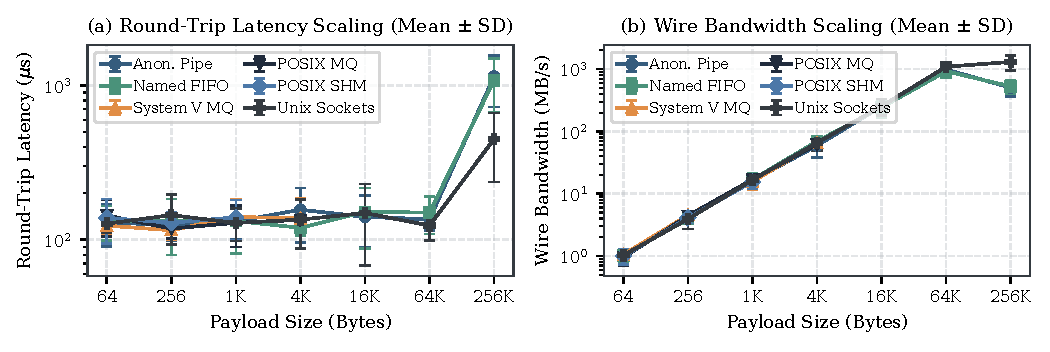
\includegraphics[height=3.8cm]{figures/latency_throughput_combined.pdf}
\caption{Empirical Performance Scaling across Classical Linux IPC Mechanisms on Fedora 45 Linux: (a) Mean Round-Trip Latency ($\mu\text{s}$) vs. Payload Size (log-log scale), and (b) Wire Data Bandwidth (MB/s) vs. Payload Size (log-log scale).}
\label{fig:latency_throughput}
\end{figure*}
